\documentclass{beamer}\usepackage[]{graphicx}\usepackage[]{color}
%% maxwidth is the original width if it is less than linewidth
%% otherwise use linewidth (to make sure the graphics do not exceed the margin)
\makeatletter
\def\maxwidth{ %
  \ifdim\Gin@nat@width>\linewidth
    \linewidth
  \else
    \Gin@nat@width
  \fi
}
\makeatother

\definecolor{fgcolor}{rgb}{0.345, 0.345, 0.345}
\newcommand{\hlnum}[1]{\textcolor[rgb]{0.686,0.059,0.569}{#1}}%
\newcommand{\hlstr}[1]{\textcolor[rgb]{0.192,0.494,0.8}{#1}}%
\newcommand{\hlcom}[1]{\textcolor[rgb]{0.678,0.584,0.686}{\textit{#1}}}%
\newcommand{\hlopt}[1]{\textcolor[rgb]{0,0,0}{#1}}%
\newcommand{\hlstd}[1]{\textcolor[rgb]{0.345,0.345,0.345}{#1}}%
\newcommand{\hlkwa}[1]{\textcolor[rgb]{0.161,0.373,0.58}{\textbf{#1}}}%
\newcommand{\hlkwb}[1]{\textcolor[rgb]{0.69,0.353,0.396}{#1}}%
\newcommand{\hlkwc}[1]{\textcolor[rgb]{0.333,0.667,0.333}{#1}}%
\newcommand{\hlkwd}[1]{\textcolor[rgb]{0.737,0.353,0.396}{\textbf{#1}}}%
\let\hlipl\hlkwb

\usepackage{framed}
\makeatletter
\newenvironment{kframe}{%
 \def\at@end@of@kframe{}%
 \ifinner\ifhmode%
  \def\at@end@of@kframe{\end{minipage}}%
  \begin{minipage}{\columnwidth}%
 \fi\fi%
 \def\FrameCommand##1{\hskip\@totalleftmargin \hskip-\fboxsep
 \colorbox{shadecolor}{##1}\hskip-\fboxsep
     % There is no \\@totalrightmargin, so:
     \hskip-\linewidth \hskip-\@totalleftmargin \hskip\columnwidth}%
 \MakeFramed {\advance\hsize-\width
   \@totalleftmargin\z@ \linewidth\hsize
   \@setminipage}}%
 {\par\unskip\endMakeFramed%
 \at@end@of@kframe}
\makeatother

\definecolor{shadecolor}{rgb}{.97, .97, .97}
\definecolor{messagecolor}{rgb}{0, 0, 0}
\definecolor{warningcolor}{rgb}{1, 0, 1}
\definecolor{errorcolor}{rgb}{1, 0, 0}
\newenvironment{knitrout}{}{} % an empty environment to be redefined in TeX

\usepackage{alltt}

\def\currentCourse{An introduction to graph analysis and modeling}
\def\currentInstitute{MSc in Statistics for Smart Data -- ENSAI}
\def\currentLogo{logo_ensai}
\def\currentDate{Automn semester, 2018}
\def\currentChapter{Introduction}


% THEME BEAMER
\usepackage{../beamer_theme}

\graphicspath{{figures/},{../common_figs/}}

\usepackage{multirow}
\usepackage{tikz}
\usepackage[vlined]{algorithm2e}

\pgfdeclareimage[width=.5cm]{computer}{computer.png}

% \usetikzlibrary{calc,shapes,backgrounds,arrows,automata,shadows,positioning}
% \tikzstyle{every state}=[fill=red,draw=none,scale=0.7,font=\small,text=white]
% \tikzstyle{every edge}=[-,shorten >=1pt,auto,thin,draw]
% \tikzstyle{alertstate}=[fill=bleu]
% \definecolor{genecolor}{RGB}{94,135,173}

\title{\currentCourse}

\subtitle{\huge\currentChapter\normalsize}

\institute{\currentInstitute}

\date{\currentDate}



\AtBeginSection{
  \begin{frame}<beamer>
    \frametitle{Outline}
    \framesubtitle{\insertpart}
    \tableofcontents[currentsection,currentsubsection, subsectionstyle=show/shaded/hide]  
  \end{frame}
}

\AtBeginSubsection{
  \begin{frame}<beamer>
    \frametitle{Outline}
    \framesubtitle{\insertpart}
    \tableofcontents[currentsection,currentsubsection, subsectionstyle=show/shaded/hide]  
  \end{frame}
}

\AtBeginSubsubsection{
  \begin{frame}<beamer>
    \frametitle{Outline}
    \framesubtitle{\insertpart}
    \tableofcontents[currentsection,currentsubsection, subsectionstyle=show/shaded/hide]  
  \end{frame}
}

\newcommand{\dotitlepage}{%
  \begin{frame}
    \titlepage
    \vfill
    \begin{center}
        \scriptsize\url{https://github.com/jchiquet/CourseStatNetwork}
    \end{center}
    \vfill
    \includegraphics[width=2cm]{\currentLogo}\hfill
    
\includegraphics[width=2.5cm]{logo_inra}
  \end{frame}
  %
}

\newcommand{\dotoc}{%
  \begin{frame}
    \frametitle{Outline}
    \tableofcontents[currentsection,
    sectionstyle=show/show,
    subsectionstyle=hide]
  \end{frame}
  %
}

\usetikzlibrary{calc,shapes,backgrounds,arrows,automata,shadows,positioning}
\IfFileExists{upquote.sty}{\usepackage{upquote}}{}
\begin{document}

\dotitlepage

\pgfdeclareimage[height=70px]{julien}{figures/julien.jpeg}

\begin{frame} 
  \frametitle{Teacher}

\begin{columns}
\hspace{1em}\begin{column}{.66\textwidth}
\begin{block}{UMR 518 AgroParisTech/Inra}
\url{https://www6.inra.fr/mia-paris} 
\end{block}
\end{column}
\begin{column}{.33\textwidth}

\includegraphics[width=2cm]{logo_inra}
\end{column}
\end{columns}

\vfill

\begin{columns}
  \hspace{1em}
  \hfill
  \begin{column}{.3\paperwidth}
    \alert{\footnotesize Julien Chiquet}\\[1ex]
    
    \pgfuseimage{julien}
    
    {\tiny Researcher at Inra}
  \end{column}
  
\end{columns}

\hfill

\begin{center}
\url{julien.chiquet@inra.fr}
\end{center}

\end{frame}

% \begin{frame}
%   \frametitle{Motivation}
%   \framesubtitle{Unravel the latent organization of an observed network}
% 
%   \begin{columns}
%     \begin{column}{.4\textwidth}
%       \begin{block}{E. coli regulatory network}
%         \begin{itemize}
%         \item relationships between gene and their products
%         \item inhibition/activation
%       \end{itemize}
%       \end{block}
%     \end{column}
%     \begin{column}{.55\textwidth}
%       \includegraphics<1>[width=\textwidth]{figures/net_reg_ecoli}
%     \end{column}
%   \end{columns}
% 
% \end{frame}

\begin{frame}
  \frametitle{Motivation}
  \framesubtitle{Unravel the latent organization of an observed network}

  \begin{figure}
    \centering
    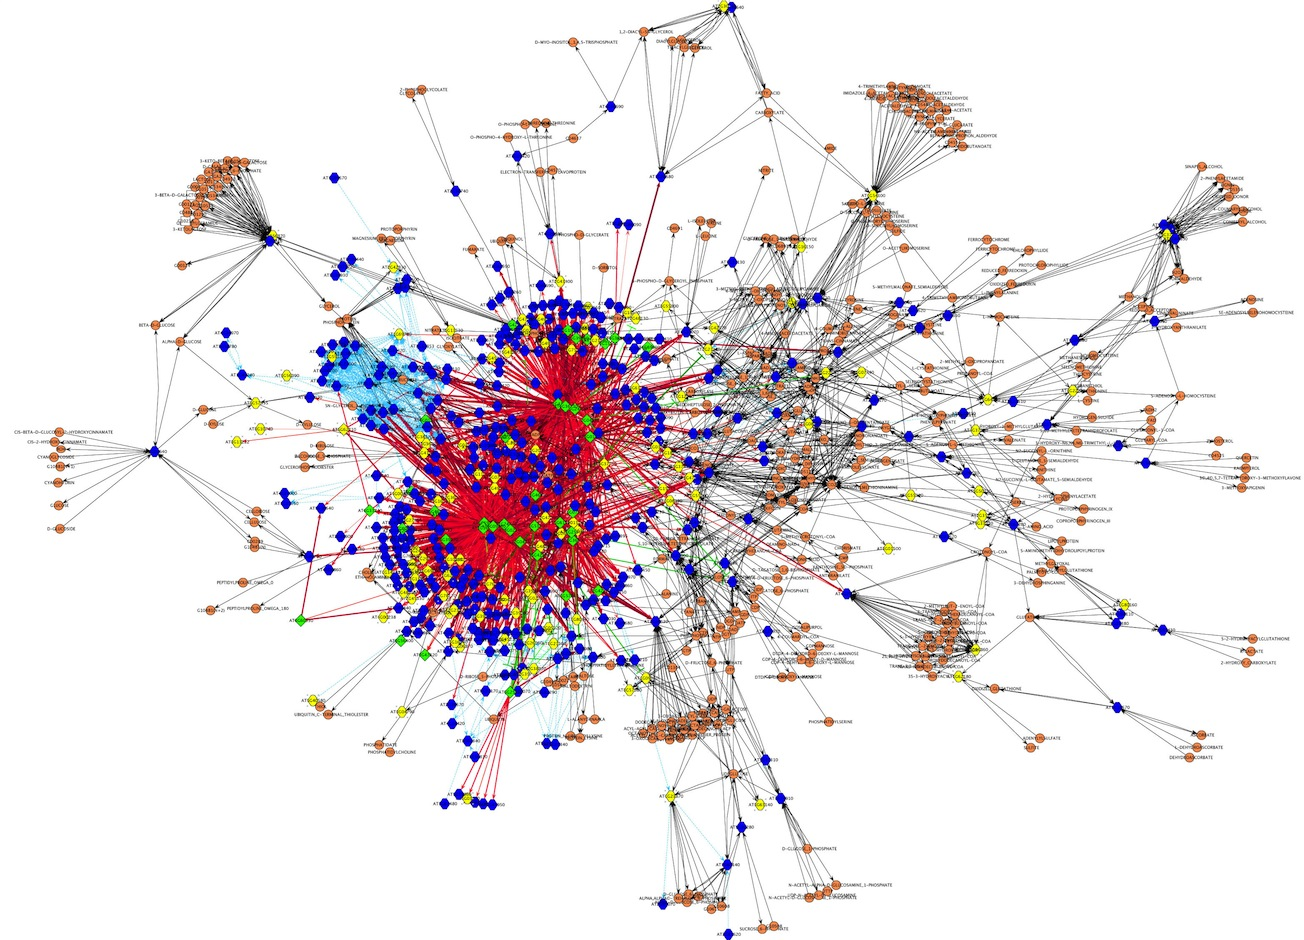
\includegraphics[width=.8\textwidth]{figures/net_reg_mamalians}
    \caption{\small Regulatory network  identified in mammalian cells:
      \alert{highly organized}}
  \end{figure}
\end{frame}

\begin{frame}
  \frametitle{Motivation}
  \framesubtitle{Unravel the latent organization of an observed network}

  \begin{figure}
    \centering
    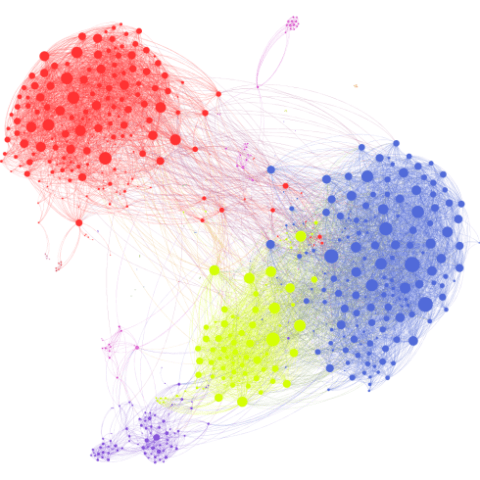
\includegraphics[width=.5\textwidth]{figures/facebook_network}
    \caption{\small Friendship network in Facebook
      \alert{communities}}
  \end{figure}
\end{frame}

\begin{frame}
  \frametitle{Motivation}
  \framesubtitle{Unravel the latent organization of an observed network}

  \begin{figure}
    \centering
    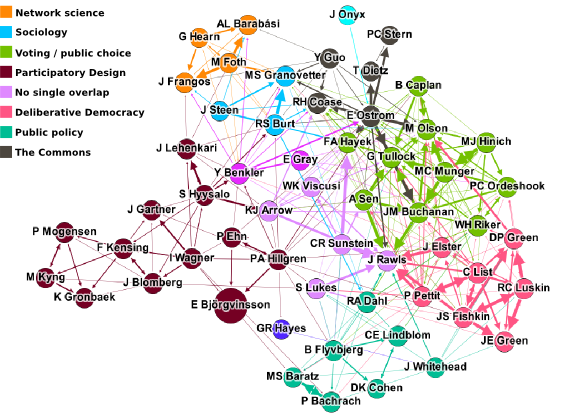
\includegraphics[width=.8\textwidth]{figures/scholar_network}
    \caption{\small Coauthorship network in google scholar
      \alert{stars + communities}}
  \end{figure}
\end{frame}

% \pgfdeclareimage[width=.3\textwidth]{affymetrix}{figures/affy}
% \pgfdeclareimage[width=.18\textwidth]{sequencer}{figures/sequencer}
% \definecolor{genecolor}{RGB}{94,135,173}
% \begin{frame}
%   \frametitle{Motivation 2}
%   \framesubtitle{Reconstruct   an   network   to   capture   important
%     features of a system}
% 
% 
%         \begin{tikzpicture}
%         \node[scale=0.75,opacity=0.75] at (-3,3) {\pgfuseimage{sequencer}};
%         \node[scale=0.75] at (-3.5,1) {\pgfuseimage{affymetrix}};
%         \node[scale=0.75,fill=red, text=white,single arrow] 
%         (inference) at (-1.7,1.7) {\sf \scriptsize Inference}; 
%         
%         \node at (-3,-0.5) {\begin{tabular}{@{}c@{}}
%             \tiny $\approx$ 10s/1000s assays \\ 
%             \tiny $\approx $ 1000/100,000s features \\
%           \end{tabular}
%         };
%         
%         %% UN GRAPH 
%         \tikzstyle{every edge}=[-,>=stealth',shorten >=1pt,auto,thin,draw,color=genecolor]
%         \tikzstyle{every node}=[fill=genecolor]
%         \tikzstyle{every state}=[draw=none,text=white,scale=0.5, transform shape] 
%         
%         % premier cluster
%         \node[state] (A1) at (0,1.75) {g1};
%         \node[state] (A2) at (1,0.75) {g2};
%         \node[state] (A3) at (0,-.25) {g3};
%         \node[state] (A4) at (-1,0.75) {g4};
%         \node[state] (A5) at (0,0.75) {g5};
%         
%         \foreach   \name/\angle/\text   in  {B1/234/g6,   B2/162/g7,
%           B3/90/g8, B4/18/g9, B5/-54/g10} {
%           \node[state,xshift=4cm,yshift=4cm]     (\name)    at
%           (\angle:1cm) {\text}; }
%         
%         \node[state] (B6) at (2,2) {g11};
%         \node[state] (C1) at (3,0.5) {g12};
%         \node[state] (C2) at (2.2,0) {g13};
%         
%         \path 
%         (A5) edge [bend left] (A1)
%         (A5) edge [bend left] (A2)
%         (A5) edge [bend left] (A3)
%         (A5) edge [bend left] (A4)
%         (B6) edge [bend right] (B1) 
%         (B6) edge [bend right] (B2) 
%         (B6) edge [bend right] (B3) 
%         (B6) edge [bend right] (B4) 
%         (B6) edge [bend right] (B5) 
%         (C2) edge [bend left] (C1)
%         (A5) edge [bend left] (B6)
%         (B6) edge [bend right] (C2);
%       \end{tikzpicture}
% 
% \end{frame}

\begin{frame} 
  \frametitle{Agenda (expected\dots)}

  \begin{description}
  \item[first day] Descriptive Analysis of Network Data (06/11)
    \begin{enumerate}
    \item \alert{Basic on Graphs} 
    \item \alert{Descriptive Statistics} 
    \item \alert{Graph Partionning} 
    \end{enumerate}

  \bigskip

  \item[second day] Statistical Models for Networks Data (15/11)
    \begin{enumerate}
    \item \alert{Stochastic Block Model} 
    \end{enumerate}

  \bigskip

  \item[third day] Extensions of the SBM and project preparation (22/11)
    \begin{enumerate}
    \item \alert{Accouting for covariates} 
    \item \alert{Weighted network} 
    \item \alert{Dynamic network} 
    \item \alert{... and more} 
    \end{enumerate}

  \end{description}
    
  \end{frame}

  \begin{frame}
    \frametitle{Module Assessment}

\begin{enumerate}
\item \alert{Practicals}

\begin{itemize}
\item each session comes with practicals on \texttt{R}
\item send me a \texttt{R}-markdown report \alert{at the end of the session/day}
\end{itemize}
\bigskip

\item \alert{Projects}
  
\begin{itemize}
\item article review (an SBM extension)
\item application project (find some network data to play with)
\item implementation of an algorithm / analysis
\end{itemize}

\end{enumerate}
       
\end{frame}
  
  \begin{frame}
    \frametitle{General books in Statistical Learning and networks}

    \url{https://github.com/jchiquet/CourseStatNetwork} 

    \vfill
    
    \begin{thebibliography}{99}
      \setbeamertemplate{bibliography item}[book]

    \bibitem[EK]{EK} Statistical Analysis of Network Data: Methods and Models, by \textcolor{black}{Eric Kolazcyk}
    \bibitem[EKGC]{EKGC} Statistical Analysis of Network Data with R, \textcolor{black}{Eric Kolazcyk and Gábor Csárdi}
    \bibitem[CB]{CB} Pattern recognition and Machine Learning, \textcolor{black}{C. Bishop}
    
    \end{thebibliography}

  \end{frame}

  % \begin{frame}
  %   \frametitle{Specific papers on more precise points}
  % 
  %   \begin{thebibliography}{99}
  %     \setbeamertemplate{bibliography item}[article]
  % 
  %   \bibitem[DPR]{DPR} A mixture model for random graphs, \textcolor{black}{Daudin, Picard, Robin}
  %   \bibitem[vL]{vL} A tutorial on Spectral Clustering, \textcolor{black}{U. von Luxburg}
  %   \bibitem[EK]{EK}  High-dimensional graphs  and variable  selection
  %     with the Lasso, \textcolor{black}{Meinshausen, B\"uhlmann}
  %   \bibitem[CB]{CB} Model Selection Through Sparse Maximum Likelihood Estimation, \textcolor{black}{Banerjee, El Gaouhi, d'Aspremont}
  %   \bibitem[EI]{EI} Sparse inverse covariance estimation with the graphical-Lasso\textcolor{black}{Hastie, Tibshirani, Friedman}
  %   \end{thebibliography}
  % 
  % \end{frame}
\end{document}
